\chapter{Implementierung}\label{ch:impl}

\sectionOG{Spieler Steuerung}\label{sec:4_SpielerSteuerung}

Die Spieler Steuerung wird mithilfe eines Observer Patterns realisiert. Beim Laden der \josieclass{BossPlayer} Klasse wird der Spieler als Observer eingetragen:

\begin{lstlisting}[label=lst:player_control_observer,
				   language=C++,
				   firstnumber=103,
				   caption=BossPlayer als Observer eintragen ( BossPlayer.cpp )]
EventDispatcher *ed = Director::getInstance()->getEventDispatcher();
if (reg) {
	ed->addCustomEventListener("BOSS_PLAYER_LEFT", CC_CALLBACK_0(BossPlayer::moveLeft, this));
\end{lstlisting}

Die Methode \textbf{addCustomEventListener()} erwartet zwei Parameter. Den Namen auf den der Observer hören soll, und das Callback, also die Funktion die ausgeführt werden soll beim Eintreffen einer solchen Nachricht, in diesem Fall \textbf{moveLeft()}. 
Gleichbedeutend muss der Spieler auch wieder aus der Liste der Observer entfernt werden, sobald die Instanz gelöscht wird. Beides passiert über dieselbe Methode, die mit dem Parameter \textbf{false} die Einträge wieder entfernt.

Die Steuerung wird über das HUD bewerkstelligt. Um genauer zu sein in der \textbf{update()} Methode der \josieclass{BossLevelHUD}.

\begin{lstlisting}[label=lst:player_control_push_msg,
				   language=C++,
				   firstnumber=181,
				   caption=Drücken des Laufen-Buttons ( BossLevelHUD.cpp )]
void BossLevelHUD::update(float dt)
{
	EventDispatcher *ed = Director::getInstance()->getEventDispatcher();
	if (_key_left || _left->isSelected())
		ed->dispatchCustomEvent("BOSS_PLAYER_LEFT");
\end{lstlisting}

Die update Methode wird kontinuierlich aufgerufen, deshalb ist vor jedem Aufruf die Abfrage auf \textbf{isSelected()} ob der aktuelle Button gedrückt ist. Das Aktivieren des Observers ist denkbar einfach über \textbf{dispatchCustomEvent()}.



\sectionDG{Sprites}

Die grundlegende Nutzung von Sprites wird im folgenden anhand der \josieclass{Tutorial} erklärt. Es werden die Bereiche, die sehr viel Anwendung in unserem Projekt fanden, erklärt. Diese sind unter anderem: das Laden von Sprites, Verwendung des Ankerpunktes als auch die Verwendung grundsätzlicher Funktionen wie \textbf{moveBy()}.

\begin{lstlisting}[label=lst:sprite_ancerpoint,
				   language=C++,
				   firstnumber=54,
				   caption=Sprite laden ( TutorialScene.cpp )]
Sprite* josie = Sprite::create("josie/josie_static.png");
josie->setAnchorPoint(Vec2::ANCHOR_BOTTOM_LEFT);
josie->setPosition(200,45);
this->addChild(josie);
\end{lstlisting}

Die erste Zeile erstellt ein Sprite Object und gibt in der create Methode den Pfad zum zu ladenden Sprite an. Als nächstes wird der Ankerpunkt des Sprites mit dem Befehl \textbf{setAnchorPoint()} festgelegt. Durch setPosition wird die Startposition festgelegt und das Sprite im Anschluss an die Scene hinzugefügt. 

\subsection{Bewegen}

Im Anschluss soll ein Beispiel für die Verwendung von Grundfunktion zur Spritemanipulation als auch Sequenzen erläutert werden. Hierbei wird ein Beispiel aus der Klasse \josieclass{BossPlayer} verwendet.

\begin{lstlisting}[label=lst:boss_attack_sequence,
				   language=C++,
				   firstnumber=219,
				   caption=Sequence erstellen ( BossLevel.cpp )]
auto right_rotate = RotateTo::create(2.0, 30.0f);
auto right_rotate_back = RotateTo::create(0.2, 0.0f);
auto right_down = MoveTo::create(0.2,Vec2(400,100));
auto right_up = MoveTo::create(1.0,Vec2(1520,600));
auto sequence = Sequence::create(right_rotate, right_down, right_up,right_rotate_back, nullptr);
right->runAction(sequence);
\end{lstlisting}

Im ersten Schritt werden zwei RotateTo Objekte als auch zwei MoveTo Objekte erstellt. Ein Objekt ist für eine Aktion zuständig die etwas verändert, das andere stellt den Uhrsprungszustand wieder her. Beim erstellen des RotateTo Objektes werden die Zeitdauer der Rotierung und der Winkel mitgegeben. Dem MoveTo Objekt wird bei der Erzeugung die Zeitdauer der Aktion als auch ein Vector der die Zielkoordinaten beschreibt übergeben. Im Anschluss wird eine Sequenz mit dem Gewünschten Ablauf der Animation erstellt und danach ausgeführt. Folgendes, Bildhaftes Beispiel soll dies veranschaulichen. 

\begin{figure}[H]
  \centering
  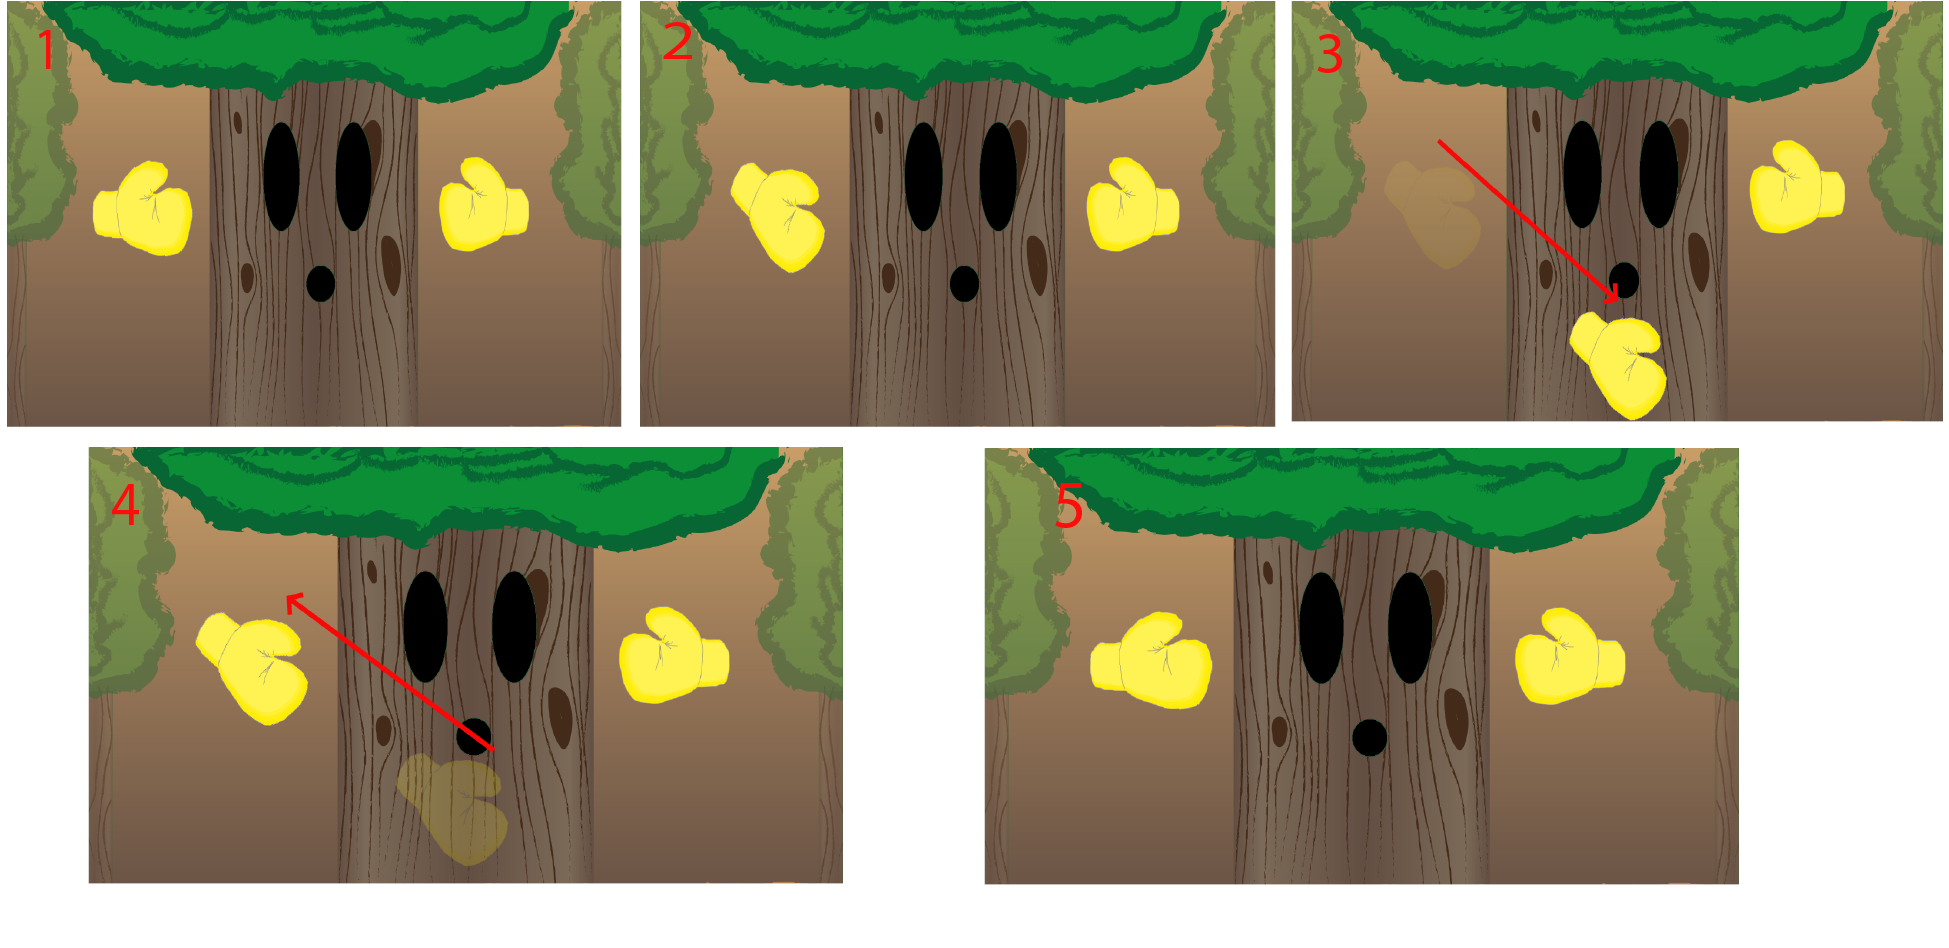
\includegraphics[width=15.5cm]{resources/dokubaum}
  \caption{Ablauf einer Sequenz}
  \label{fig:dokubaum} 
\end{figure}

\subsection{Animieren}
Eine Erklärung für den Aufbau einer Animation durch ein Spritesheet und eine .plist Datei soll durch das folgende Beispiel erbracht werden.

\begin{lstlisting}[label=lst:build_josie_animation,
				   language=C++,
				   firstnumber=53,
				   caption=Animation erstellen ( CollisionLayer.cpp )]
Vector<SpriteFrame*> frames;
SpriteFrameCache *frameCache = SpriteFrameCache::getInstance();

char file[9] = { 0 };

for (int i = 0; i < 6; i++) {
	sprintf(file, "coin%04d", i);
	SpriteFrame *frame = frameCache->getSpriteFrameByName(file);
	frames.pushBack(frame);
}

Animation *animation = Animation::createWithSpriteFrames(frames, 0.1);
\end{lstlisting}

Zu Begin erstellen wir einen String mit Hilfe eines Char Arrays und einem Vector zur Erstellung von Frames. In der SpriteFrameCache Instanz sind bereits alle Spritesheets geladen. Die nachfolgende Schleife iteriert durch die benötigten Bildnamen um diese zum Array hinzuzufügen. Hierbei ist zu beachten dass Für eine Animation mehrere Bilder nacheinander geladen werden müssen, diese haben die Namenskonvention "'coin0000"', "'coin0001"' etc. Der SpriteFrame mit dem generierten Bildnamen wird aus dem SpriteFrameCache geladen und in den anfangs definierten Vektor eingefügt. 
Sobald die For-Schleife abgearbeitet ist, wird eine Animation mithilfe \textbf{createWithSpriteFrames()} erstellt. Dieser wird der Vektor und eine Verzögerung zwischen den Frames übergeben.

\begin{lstlisting}[label=lst:build_josie_animation_reverse,
				   language=C++,
				   firstnumber=96,
				   caption=Sequence Umkehren ( LevelPlayer.cpp )]
startRunningAfterAnimation(animationWithFrame("josiejump", 6, 0.0001)->reverse())
\end{lstlisting}

Die Methode animationWithFrame liefert eine Animation zurück. Darauf wird die Methode \textbf{reverse()} aufgerufen, welche die Animation rückwärts ablaufen lässt.

\begin{figure}[H]
  \centering
  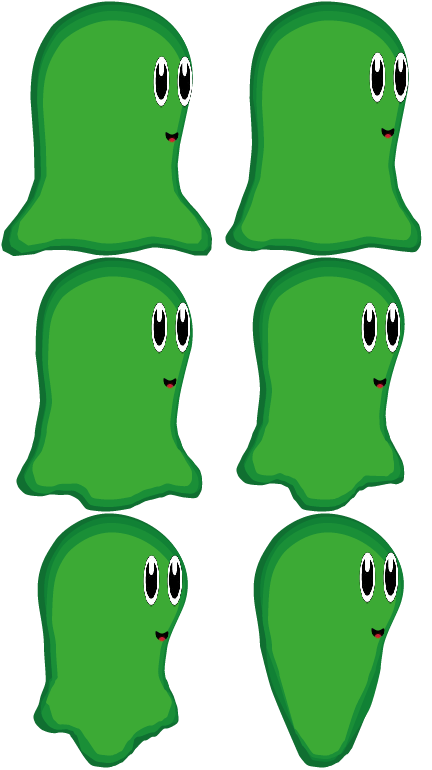
\includegraphics[height=5cm]{resources/josiejump}
  \caption{Die Sprung-Animation in einzelnen Sprites}
  \label{fig:josie_jump} 
\end{figure}


\subsection[Fortsetzung des Programmablaufs]{Fortsetzung des Programmablaufs \scriptsize Oleg Geier}

Manchmal ist es sinnvoll eine Funktion auszuführen sobald eine Animation beendet ist. Hierfür wird ein Callback erstellt und in eine \cocosclass{CallFuncN} gekapselt.

\begin{lstlisting}[label=lst:CallFuncN,
				   language=C++,
				   firstnumber=116,
				   caption=startRunningAfterAnimation ( LevelPlayer.cpp )]
CallFuncN *call = CallFuncN::create(
	CC_CALLBACK_0(LevelPlayer::startRunningCallback, this));
Sequence *seq = Sequence::createWithTwoActions(animation, call);
spriteImage->runAction(seq);
\end{lstlisting}

In diesem Beispiel wird die Animation für das Stoppen von Josie und anschließend die Methode \textbf{startRunningCallback()} ausgeführt. '\texttt{this}' ist die aktuelle Player Instanz.



\sectionDM{AudioUnit}\label{sec:4_Audiounit}
Die Klasse \josieclass{AudioUnit} kümmert sich um das Laden, Abspielen, Pausieren und Enfernen der Audiodateien. Hierbei handelt es sich durchgehend um statische Funktionen, sodass man die Klasse nicht erst instanziieren muss, sondern die Funktionen einfach von Außerhalb mit \josieclass{AudioUnit::} aufrufen kann.

\subsection{Laden von Soundeffekten}
Ein wichtiger zu beachtender Aspekt bei Spielen mit vielen Soundeffekten ist die Notwendigkeit des vorangehenden Ladens dieser. Falls man dies nicht tut, kann es zu Performance-Problemen kommen. Der Grund dafür ist, dass zum Beispiel beim Drücken des "'Sprung"'-Buttons jedesmal beim Ausführen, der Sound erst geladen, abgespielt und anschließend wieder aus dem Speicher entfernt werden würde. Deshalb wird zum Beispiel beim Erstellen des \josieclass{BossLevel} im Konstruktor die Funktion \josieclass{AudioUnit::preloadBossSounds()} aufgerufen.

\begin{lstlisting}[label=lst:preloadBossSounds,
				   language=C++,
				   firstnumber=30,
				   caption=BossLevel-Sounds laden ( AudioUnit.cpp )]
void AudioUnit::preloadBossSounds()
{
	SimpleAudioEngine* engine = SimpleAudioEngine::getInstance();
	engine->setEffectsVolume(UserDefault::getInstance()
						->getIntegerForKey("sfx_volume")/200.0);
	engine->preloadEffect("audio/boss_sounds/boss_hit1.mp3");
	//Weitere Preloads
}
\end{lstlisting}

An dieser Stelle sei erwähnt dass ganze Musiktitel, wie zum Beispiel die Hintergrundmusik, nicht zwingend geladen werden müssen da diese nicht öfter hintereinander abgespielt, sondern wenn nötig geloopt werden. 

Die Methode \textit{unloadBossSounds} gleicht der Methode zum Laden der Sounds. Der einzige Unterschied ist, dass \textbf{unloadEffect} anstelle von \textbf{preloadEffect} verwendet wird.

Gleichzeitig mit dem Laden der Sounds wird die Lautstärke der Effekte auf den in \cocosclass{UserDefault} gespeicherten integer--Wert mit dem Key "'sfx\_volume"' gesetzt. Dieser wird durch einen individuellen double--Wert (in diesem Fall 200.0) geteilt, da die \textbf{setEffectsVolume} Methode nur double--Werte akzeptiert. Die Möglichkeit Einstellungen für Musik- und SFX-Lautstärke im Spiel selbst vorzunehmen, ist durch die Klasse \josieclass{OptionScreen} realisiert. 

Innerhalb der \josieclass{AudioUnit} wird auf die Singleton-Instanz der \cocosclass{SimpleAudioEngine}, die alle nötigen Funktionen liefert, zugegriffen. So gesehen ist die \josieclass{AudioUnit} ein Wrapper der die Verwendung von Audio im Code der anderen Klassen erheblich erleichtert und zusätzlich zu "'saubererem"' Code führt. 



\subsection{Abspielen von Soundeffekten und Musik} 
Um nun einen Sound-Effekt abzuspielen, ruft man an passender Stelle die gewünschte Methode auf. Als Beispiel ist das Abspielen des Sounds gegeben, den man hört wenn der \josieclass{BossPlayer} getroffen wird.

\begin{lstlisting}[style=singleline]
AudioUnit::playJosieHitSound();
\end{lstlisting}

Die Logik hinter der Funktion ist relativ simpel. Es existieren drei verschiedene Sound-Effekte die mit Hilfe eines String-Ersetzers und einer Zufallszahl zwischen eins und drei zufällig ausgewählt und abgespielt werden. Die übergebenen Parameter an die Methode \textbf{playEffect} sind der Pfad der Audiodatei, Loop, Pitch, Pan, Gain.

\begin{lstlisting}[label=lst:playJosieShootSound,
				   language=C++,
				   firstnumber=30,
				   caption=BossLevel Shoot Sound abspielen ( AudioUnit.cpp )]
void AudioUnit::playJosieHitSound()
{
	std::ostringstream s;
	s << "audio/josie_sounds/josie_hit"<< (rand()%3)+1 <<".mp3";

	SimpleAudioEngine* engine = SimpleAudioEngine::getInstance();
	engine->playEffect(s.str().c_str(), false, 1.0, 1.0, 0.7);
	
}
\end{lstlisting}

Analog kann das ganze auf das Abspielen der Hintergrundmusik übertragen werden, wobei dann auf den String-Ersetzer verzichtet und der Pfad hard gecoded wird. Außerdem wird die Zufallsfunktion überflüssig da es die Hintergrundsongs nur einmal gibt und die Parameter Pitch,Pan und Gain fallen weg.



\sectionOG{CollisionLayer}\label{sec:4_CollisionLayer}

Das \josieclass{CollisionLayer} kümmert sich ausschließlich um die Kollision von Objekten. Die Kollision zum Boden wird im \href{sec:4_Kollisionsabfrage}{nächsten Kapitel} erläutert. Alle Interaktiven Elemente im Spiel besitzen Kollision, dazu zählt der Spieler, Boss Gegner, Münzen, Geschoss Kugeln und herabfallende Stachelbeeren.

\subsection{Debugging Optionen}\label{sec:CollisionLayerDebug}

Zu Debugging Zwecken kann die \josieclass{CollisionLayer} Klasse den Bereich der Kollision grafisch hervorheben.

\begin{figure}[H]
  \centering
  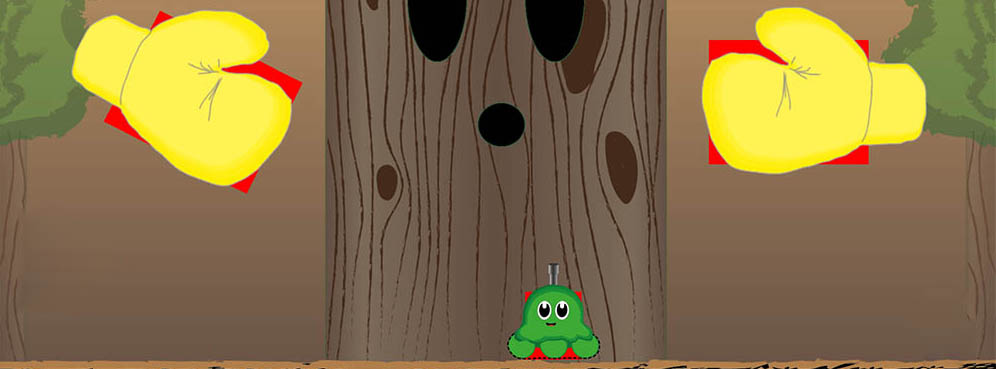
\includegraphics[width=\textwidth - 50pt]{resources/CollisionLayer_BossKampf.jpg}
  \caption{CollisionLayer Debug im Boss Kampf}
  \label{fig:collision_debug_boss} 
\end{figure}

Wenn man genau hinsieht erkennt man, dass auch Münzen über eine Kollision verfügen. Tödliche Objekte in der Karte (bsp. Dornen) jedoch nicht.

\begin{figure}[H]
  \centering
  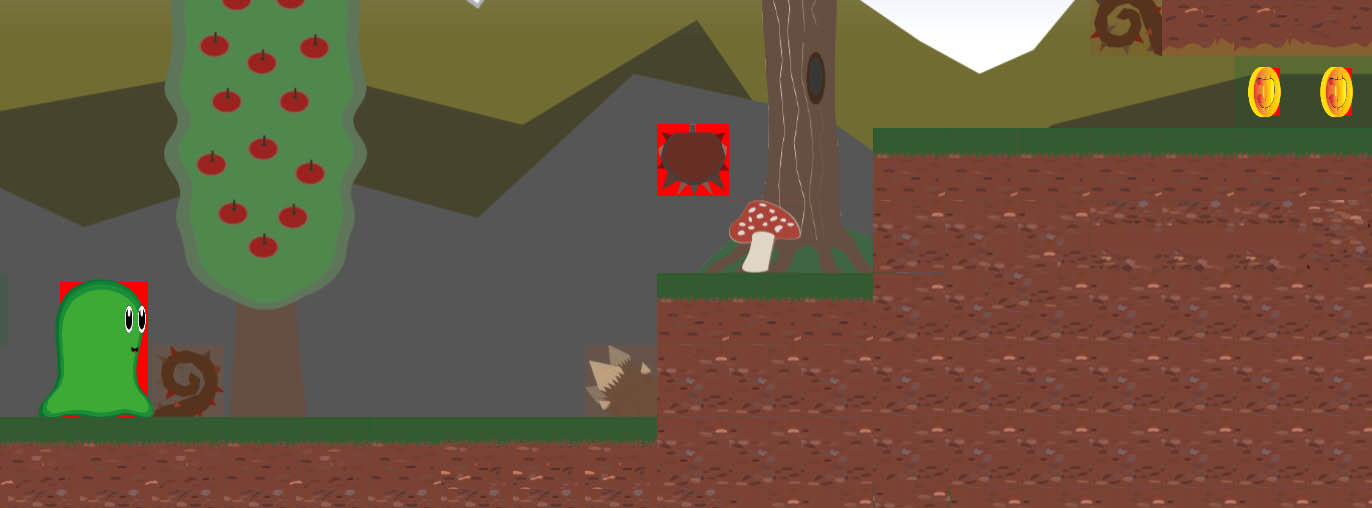
\includegraphics[width=\textwidth - 50pt]{resources/CollisionLayer_Level}
  \caption{CollisionLayer Debug im Level}
  \label{fig:collision_debug_level} 
\end{figure}


\subsection{Listener registrieren}

Die Klasse verfügt über eine Funktion \textbf{setCollisionListener(CollisionLayer*)} die ein anderes Collision Layer als Parameter erwartet. Dabei wird das übergebene Objekt in einer internen Variable gespeichert und in der \textbf{update()} Methode kontinuierlich auf Kollision überprüft.

\subsection{Gegenseite Collision Notification}

Sobald eine Kollision festgestellt wird, werden beide Objekte darüber informiert. Die Methode \textbf{hitByCollision(CollisionLayer*)} ist in der \josieclass{CollisionLayer} Klasse nicht implementiert und muss von den einzelnen Subklassen durch Logik ergänzt werden.

So wird bei einem \josieclass{StageHazard} - im Falle einer Collision mit dem Spieler - das tödliche Objekt wieder auf Anfang positioniert.

\begin{lstlisting}[label=lst:hit_by_collision,
				   language=C++,
				   firstnumber=32,
				   caption=Collision Notification ( StageHazard.cpp )]
void StageHazard::hitByCollision(CollisionLayer* other)
{
	if (other->collisionType == CollisionLayerTypeLevelPlayer) {
		this->fallDown();
	}
}
\end{lstlisting}



\sectionOG{Kollisionsabfrage zum Boden}\label{sec:4_Kollisionsabfrage}

Die Kollisionsabfrage ist auf den ersten Blick nicht sofort einleuchtend. Prinzipiell wird für die komplette Karte ein Array mit ganzzahligen Werten angelegt, also für jede Spalte (72px breite, vertikale Linie auf dem Bildschirm) wird ein \textbf{long} Wert gespeichert.
Die Karte ist 15 Tiles hoch. Für jedes Tile wird ein Bitwert gesetzt ob Kollision besteht.

\begin{lstlisting}[label=lst:collision_detection,
				   language=C++,
				   firstnumber=271,
				   caption=Collision Column abfragen ( MapController.cpp )]
long MapController::getColumnBitmapForGID(int x, int tile_gid)
{
	TMXLayer *meta = getLayer("Meta_layer");
	long col=0;
	for (int i=_mapSize.height; i>0; i--) {
		col<<=1;
		int gid = meta->getTileGIDAt(Vec2(x,i-1));
		col |= (gid==tile_gid);
	}
	return col;
}
\end{lstlisting}

Die Schleife durchläuft - von unten angefangen - alle Tiles einer Spalte und fragt ab, ob das Kollisions Attribut gesetzt ist. Bei jedem Schleifendurchlauf wird der Bit-Shift-Operator (\texttt{<<}) angewandt, sodass das höher liegende Tile hinten angefügt wird. Das Anfügen geschiet mit dem Oder-Operator und der gleichzeitigen Zuweisung (\texttt{|=}).

Der abschließende \texttt{long} Wert weißt an dem höchstwertigen Bit die Kollision für das unterste Teil auf und am niedrig wertigsten Bit die Kollision für das Tile am oberen Bildschirmrand.

Dieselbe Bitmap wird auch für tödliche Kollision in einem separaten Array erstellt. Beides geschiet nur beim Laden der Karte. Für die tatsächliche Kollisionsabfrage wird nur noch auf diese Bitmap zugegriffen.


\sectionJK{Automatisch erzeugte Tilemaps}\label{sec:4_Automatisch erzeugte Tilemapst}

Die  \josieclass{TMXEdit} Klasse hat die Aufgabe, abhängig von einem übergebenen Schwierigkeitsgrad, automatisch einen Level zu generieren. Drei Aspekte waren dabei besonders wichtig: Ein erzeugter Level sollte fordernd sein, er sollte Abwechslungsreich sein und er sollte – unabhängig davon, wie die Zufallsparameter ausfallen – keine Stellen beinhalten, die unmöglich zu bewältigen sind. Zusätzlich war es wünschenswert, dass der Spieler alle Münzen, welche im Level platziert sind erreichen kann.


\subsection{Generieren des Levels}
Das Grundgerüst des Zufallslevels ist immer identisch. Die ersten 20 Tiles stellen nie ein Hindernis dar, die letzten 38 sind das Levelende, welches in jedem Level gleich aussieht. Aus diesem Grund laden alle automatisch erzeugten Level die gleiche Tilemap, welche diesen Aufbau bereits umsetzt, und befüllen diese dann zur Laufzeit.
Zum Befüllen des Levels wird dieses von Anfang bis Ende durchlaufen.  Dabei werden in zufälliger Reihenfolge Funktionen aufgerufen, welche Abschnitte des Levels nach einem jeweils eigenen Muster erzeugen. Das tatsächliche platzieren der Tiles erfolgt durch das zuweisen der GID für die zu bearbeitenden Tilemap-Koordinaten. 
Dir folgenden Funktionen beispielsweise füllen eine ausgewählte Spalte ab einer gewissen Höhe
nach unten komplett mit Boden-Tiles und einem Gras-Tile an oberster Stelle.
\begin{lstlisting}[label=lst:place_ground,
				   language=C++,
				   firstnumber=127,
				   caption=Platzieren von Boden-Tiles ( TMXEdit.cpp )]
void TMXEdit::placeGround(int x, int y) {

	_backgroundLayer->setTileGID(TOPDIRT[arc4random() % 4], Vec2(x, y));
	_metaLayer->setTileGID(COLLIDE, Vec2(x, y));
	if (y < _minheight)
		placeDirt(x, y + 1);
}

void TMXEdit::placeDirt(int x, int y) {
	_backgroundLayer->setTileGID(DIRT[arc4random() % 4], Vec2(x, y));
	_metaLayer->setTileGID(COLLIDE, Vec2(x, y));
	if (y < _minheight)
		placeDirt(x, y + 1);
}

}
\end{lstlisting}

Ein einfaches Beispiel um zu erklären, wie Abschnitte nach einem gewissen Muster erzeugt werden findet man in der folgenden Funktion, welche im Level eine oder mehrere aufeinander folgende  schwebenden Plattformen erzeugt. Wie alle Funktionen die gesamte Abschnitte erzeugen, verfügt sie über einen ganzzahligen Rückgabewert. Dieser gibt an, bis zu welcher Spalte die Funktion die Tilemap bearbeitet hat.
\begin{lstlisting}[label=lst:make_floating,
				   language=C++,
				   firstnumber=171,
				   caption=Abschnitt mit schwebenden Plattformen erzeugen( TMXEdit.cpp )]
int TMXEdit::makeFloating(int x, int height) {
	x += _minJumpDistance + arc4random() % _maxJumpDistance-1;
	int done = x + _partlength * (1 + arc4random() % 2);
	while (x <= done) {
		x = FloatingPlatform(x, height, 3+arc4random()%3);
		x += _minJumpDistance + arc4random() % _maxJumpDistance;
	}
	return x;
}
\end{lstlisting}
Zu Beginn der Funktion wird eine gewisse Anzahl an Spalten übersprungen. Die so entstehende Lücke wird in ihrer Weite durch den Schwierigkeitsgrad definiert (dieser beeinflusst die variablen \_minJumpDistance und \_maxJumpDistance). Anschließend wird bestimmt, wie lang der aktuelle Abschnitt sein soll. Die Variable „done“ legt fest, bis zu welcher x-Koordinate ein neues Element(hier: eine einzelne schwebende Plattform) dieses Abschnitts Angefangen werden kann. Die Plattform selbst wird hier durch eine andere Funktion erzeugt. Diese weißt der Reihe nach den Kacheln auf der übergebenen Höhe die jeweiligen GIDs zu. Die Länge der Plattform ist ebenfalls ein Parameter, welcher hier durch einen Zufallswert geliefert wird. 
Die Wahl der einzelnen Levelbausteine erfolgt in Form eines Switch-Statements. Der übergebene Ausdruck ist dabei selbstverständlich ein Zufallswert, durch ihn wird bestimmt, welcher Abschnitt als nächstes generiert werden soll. Durch das wiederholen dieses switch Befehls in einer Schleife kann so der gesamte Level zufällig aufgefüllt werden.


\subsection{Platzieren der Münzen}
Neben dem Erstellen des Levels gibt es noch ein zweites Problem das bewältigt werden musste. Die Münzen mussten im Level verteilt werden – in erreichbaren Positionen, abhängig vom Aufbau des Levels.
Dafür zuständig ist folgende Funktion (sowie die von ihr aufgerufenen):

\begin{lstlisting}[label=lst:place_coins,
				   language=C++,
				   firstnumber=171,
				   caption=Automatisches Platzieren von Münzen( TMXEdit.cpp )]
void TMXEdit::placeCoins(int number) {
	int counter = 0;
	int distance = (int) map->getMapSize().width/number;
	int x = 50;
	while (counter < number) {
		int y = isSafe(x);
		if (y > 0) {
			placeCoin(x, y);
			counter++;
			x = x - (x % distance) + distance;
			if(x >  map->getMapSize().width -50) x= 50;
		} else {
			x += 1;
		}
	}
}
\end{lstlisting}
Die Funktion stellt sicher, dass die gewünschte Anzahl an Münzen in regelmäßigen Abständen zueinander platziert wird. Durch die isSafe Funktion wird zuerst die Höhe der Umgebung an der betrachteten Position ermittelt und dann geprüft, ob die Position für den Spieler erreichbar ist, ohne zu verlieren. Ist dies nicht der Fall, so wird Spalte für Spalte überprüft, bis die Münze platziert wurde. Sollte das Ende der Karte erreicht werden, so wird die nächste Münze wieder am Anfang platziert. Ein Problem tritt dabei höchstens auf, wenn die gewünschte Anzahl an Münzen die Anzahl an sicheren Positionen übertrifft. Das Spiel würde dann eine Endlosschleife betreten.  Da eine so hohe Anzahl an Münzen jedoch ohnehin nicht wünschenswert ist- auf manchen Geräten kann dies zu Einbrüchen der Framerate führen- darf dieser Sonderfall ignoriert werden (Außerdem wäre es aus Sicht eines Game-Designers keine gute Idee, so viele Münzen verfügbar zu machen, da so das Erfolgserlebnis beim Einsammeln verloren geht).

